206. \begin{figure}[ht!]
\center{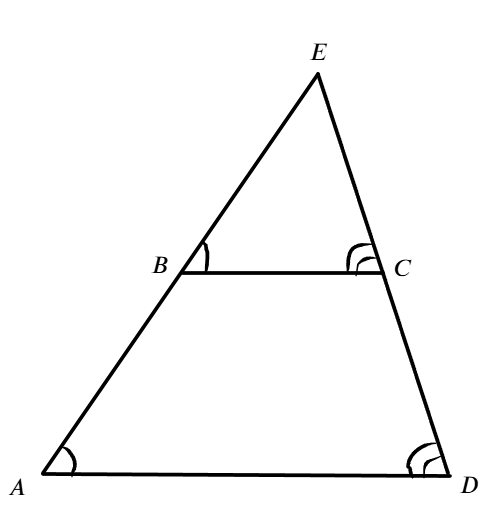
\includegraphics[scale=0.35]{g9-204.png}}
\end{figure}\\
Треугольники $BEC$ и $AED$ подобны по двум углам (соответственным при параллельных прямых $AD$ и $BC$), коэффициент подобия равен $\cfrac{BC}{AD}=
\cfrac{6}{31}.$ Тогда $\cfrac{|BE|}{|BE|+20}=\cfrac{6}{31},\ 31|BE|=6|BE|+120,\ |BE|=\cfrac{24}{5},$ а $\cfrac{|CE|}{|CE|+15}=\cfrac{6}{31},\ 31|CE|=6|CE|+90,\ |BE|=\cfrac{18}{5}.$ Таким образом, в треугольнике $BEC$ имеем равенство $|BE|^2+|CE|^2=\cfrac{576}{25}+\cfrac{324}{25}=\cfrac{900}{25}=36=|BC|^2,$ а значит треугольник $BEC$ является прямоугольным, и угол между прямыми, содержащими боковые стороны трапеции, равен $90^\circ.$\\
